% La plataforma de un vistazo: lo que entra (los dos CSV en bruto), lo que hace dentro y lo que sale (el dashboard).
% Compilar: latexmk, desde esta carpeta (el PDF va a figures/slides). La captura es figures/slides/10_dashboard.png.
\documentclass[12pt,border=14pt]{standalone}
\usepackage[T1]{fontenc}
\usepackage[utf8]{inputenc}
\usepackage[sfdefault,proportional]{inter}
\usepackage{amsmath,amssymb}
\usepackage{graphicx}
\usepackage{tikz}
\usetikzlibrary{arrows.meta,calc,patterns}
\definecolor{ink}{HTML}{111111}
\definecolor{ink2}{HTML}{3C4043}
\definecolor{muted}{HTML}{8A8F98}
\definecolor{rule}{HTML}{D9DBDF}
\definecolor{soft}{HTML}{F4F5F7}
\definecolor{cell}{HTML}{DCDFE3}
\definecolor{work}{HTML}{30A46C}
\definecolor{own}{HTML}{E5484D}
\definecolor{starved}{HTML}{F0A530}
\definecolor{blocked}{HTML}{3E8BF0}
\definecolor{nodata}{HTML}{8B8D98}
\definecolor{bezel}{HTML}{1C1F23}
% Verdes del icono de Excel
\definecolor{xlDark}{HTML}{185C37}
\definecolor{xl}{HTML}{107C41}
\definecolor{xlMid}{HTML}{21A366}
\definecolor{xlLight}{HTML}{33C481}

\tikzset{
  flow/.style={-{Stealth[length=3.2mm,width=2.4mm]}, line width=1.1pt, color=ink},
  tile/.style={fill=soft, rounded corners=7pt, draw=none},
  num/.style={font=\footnotesize\bfseries\color{muted}, anchor=west},
  head/.style={font=\large\bfseries\color{ink}, anchor=west},
  note/.style={font=\footnotesize\color{muted}, anchor=west},
  chip/.style={draw=rule, line width=0.6pt, rounded corners=2pt, fill=white, font=\scriptsize\bfseries\color{ink2}, minimum height=4.6mm, minimum width=7.4mm, inner xsep=1pt},
  % Icono de un fichero de Excel: la hoja en franjas verdes y delante el cuadrado con la X
  excel/.pic={
    \begin{scope}
      \clip[rounded corners=2.4pt] (0.48,0) rectangle (1.78,1.66);
      \fill[xlDark] (0.48,0) rectangle (1.78,0.415);
      \fill[xl] (0.48,0.415) rectangle (1.78,0.83);
      \fill[xlMid] (0.48,0.83) rectangle (1.78,1.245);
      \fill[xlLight] (0.48,1.245) rectangle (1.78,1.66);
      \fill[white, opacity=0.18] (1.13,0) rectangle (1.78,1.66);
    \end{scope}
    \fill[xl, rounded corners=2.4pt] (0,0.3) rectangle (1.06,1.36);
    \node[text=white, font=\bfseries\fontsize{20}{20}\selectfont] at (0.53,0.83) {X};
  },
}

\begin{document}
\begin{tikzpicture}[x=1cm,y=1cm]
  % Medidas: tres columnas por dos filas de bloques dentro de la caja del modelo
  \def\TW{5.4}\def\TH{3.6}\def\G{0.4}\def\P{0.5}
  \def\BX{6.4}                         % borde izquierdo de la caja
  \pgfmathsetmacro{\BW}{2*\P+3*\TW+2*\G}
  \pgfmathsetmacro{\BH}{2*\P+2*\TH+\G+0.3}
  \pgfmathsetmacro{\BR}{\BX+\BW}
  \pgfmathsetmacro{\MY}{\BH/2}

  % --- Entrada: los dos ficheros tal cual llegan -------------------------------------------
  \pic at (1.25,6.2) {excel};
  \node[font=\normalsize\bfseries\color{ink}] at (2.14,5.7) {datos\_hackaton.csv};
  \node[font=\footnotesize\color{muted}] at (2.14,5.2) {91 máquinas $\times$ 20 días};
  \foreach \c [count=\k from 0] in {TBF,TAP,DES,SAT,NAP,NPR}
    \node[chip] at (2.14+\k*0.82-2.05,4.6) {\c};
  \pic at (1.25,1.6) {excel};
  \node[font=\normalsize\bfseries\color{ink}] at (2.14,1.1) {config\_hackaton.csv};
  \node[font=\footnotesize\color{muted}] at (2.14,0.6) {orden de las 91 operaciones};
  \draw[flow] (4.55,7.03) -- (\BX,7.03);
  \draw[flow] (4.55,2.43) -- (\BX,2.43);

  % --- El modelo: caja discontinua con todo lo que pasa dentro -----------------------------
  \draw[ink2, line width=1.1pt, dash pattern=on 5pt off 3.5pt, rounded corners=12pt] (\BX,0) rectangle (\BR,\BH);
  \node[fill=white, inner xsep=7pt, font=\Large\bfseries\color{ink}, anchor=west] at (\BX+0.45,\BH) {LOSSIA};
  \node[fill=white, inner xsep=7pt, font=\footnotesize\color{muted}] at (\BX+\BW/2,0) {sin pasos manuales \;·\; misma entrada, misma salida};

  % Fondo, número y título de cada bloque. #1 columna, #2 fila (0 arriba), #3 número, #4 título, #5 nota
  \newcommand{\tile}[5]{%
    \pgfmathsetmacro{\tx}{\BX+\P+#1*(\TW+\G)}%
    \pgfmathsetmacro{\ty}{\P+0.1+(1-#2)*(\TH+\G)}%
    \fill[tile] (\tx,\ty) rectangle ++(\TW,\TH);
    \node[num] at (\tx+0.32,\ty+\TH-0.48) {#3};
    \node[head] (h) at (\tx+0.86,\ty+\TH-0.48) {#4};
    \node[note, anchor=base west] at ($(h.base east)+(0.08,0)$) {#5};
  }

  % 01 · Limpieza: la rejilla de filas, un día sin producción fuera, una columna sin dato fiable
  \tile{0}{0}{01}{Limpieza}{}
  \begin{scope}[shift={(\tx+0.2,\ty-0.98)}]
    \foreach \i in {0,...,8} \foreach \j in {0,...,3} {
      \pgfmathsetmacro{\px}{0.72+\i*0.42}\pgfmathsetmacro{\py}{1.72+\j*0.42}
      \ifnum\i=6 \fill[pattern=north east lines, pattern color=nodata] (\px,\py) rectangle ++(0.3,0.3);
      \else\ifnum\j=2 \fill[own, opacity=0.35] (\px,\py) rectangle ++(0.3,0.3);
      \else \fill[cell, rounded corners=1pt] (\px,\py) rectangle ++(0.3,0.3); \fi\fi
    }
    \fill[ink2, rounded corners=1pt] (0.72+2*0.42,1.72) rectangle ++(0.3,0.3);
    \fill[ink2, rounded corners=1pt] (0.72+4*0.42,1.72+3*0.42) rectangle ++(0.3,0.3);
    \draw[own, line width=1.2pt] (0.55,1.72+2*0.42+0.15) -- (4.45,1.72+2*0.42+0.15);
  \end{scope}

  % 02 · KPIs: el día de 22 h en cuatro estados y los indicadores del reto
  \tile{1}{0}{02}{KPIs}{}
  \begin{scope}[shift={(\tx+0.2,\ty-1.75)}]
    \def\y{3.05}
    \fill[work]    (0.5,\y) rectangle (2.25,\y+0.42);
    \fill[own]     (2.3,\y) rectangle (2.98,\y+0.42);
    \fill[starved] (3.03,\y) rectangle (3.76,\y+0.42);
    \fill[blocked] (3.81,\y) rectangle (4.5,\y+0.42);
    \foreach \x/\t in {1.375/TBF,2.64/TAP,3.395/DES,4.155/SAT} \node[font=\scriptsize\bfseries\color{ink2}] at (\x,\y-0.25) {\t};
    \node[font=\footnotesize\color{muted}, anchor=south] at (2.5,\y+0.45) {22 h al día};
  \end{scope}

  % 03 · Quién frena: las dos flechas apuntan a la estación que frena la línea
  \tile{2}{0}{03}{Quién frena}{}
  \begin{scope}[shift={(\tx+0.2,\ty-1.10)}]
    \def\y{2.35}
    \draw[rule, line width=2.5pt] (0.4,\y) -- (4.6,\y);
    \draw[blocked, line width=1.4pt, fill=blocked!12, rounded corners=3pt] (0.65,\y-0.33) rectangle ++(0.95,0.66);
    \draw[own, line width=2.2pt, fill=own!12, rounded corners=3pt] (2.02,\y-0.36) rectangle ++(0.96,0.72);
    \draw[starved, line width=1.4pt, fill=starved!14, rounded corners=3pt] (3.4,\y-0.33) rectangle ++(0.95,0.66);
    \draw[-{Stealth[length=2.6mm]}, line width=1.4pt, blocked] (1.25,\y+0.42) to[bend left=50] (2.2,\y+0.48);
    \draw[-{Stealth[length=2.6mm]}, line width=1.4pt, starved] (3.75,\y+0.42) to[bend right=50] (2.8,\y+0.48);
  \end{scope}

  % 04 · Penalización: horas propias más lo que hace perder a sus vecinas (ST-0260)
  \tile{0}{1}{04}{Penalización}{}
  \begin{scope}[shift={(\tx+0.2,\ty-1.63)}]
    \def\y{2.7}
    \fill[own]     (0.5,\y) rectangle ++(0.17,0.5);
    \fill[blocked] (0.72,\y) rectangle ++(1.7,0.5);
    \fill[starved] (2.47,\y) rectangle ++(1.05,0.5);
    \node[font=\normalsize\bfseries\color{ink}, anchor=west] at (3.6,\y+0.25) {186 h};
    \node[font=\footnotesize\color{muted}, anchor=south west] at (0.45,\y+0.52) {ST-0260};
  \end{scope}

  \tile{1}{1}{05}{Predicción}{}
  \begin{scope}[shift={(\tx+0.2,\ty-1.09)}]
    \fill[ink, opacity=0.11] (2.35,2.48) -- (4.6,3.0) -- (4.6,1.92) -- cycle;
    \fill[ink, opacity=0.14] (2.35,2.48) -- (4.6,2.74) -- (4.6,2.18) -- cycle;
    \draw[ink, line width=1.2pt, line join=round] (0.5,2.25) -- (0.85,2.62) -- (1.2,2.32) -- (1.55,2.5) -- (1.95,2.2) -- (2.35,2.48);
    \foreach \p in {(0.5,2.25),(0.85,2.62),(1.2,2.32),(1.55,2.5),(1.95,2.2),(2.35,2.48)} \fill[ink] \p circle (1.6pt);
    \fill[ink] (2.95,2.5) circle (1.9pt);
    \fill[ink] (3.5,2.38) circle (1.9pt);
    \draw[own, line width=0.8pt, dash pattern=on 1.5pt off 1.5pt] (3.95,2.86) -- (3.95,3.28); \fill[own] (3.95,3.3) circle (2.8pt);
    \fill[own] (4.42,3.3) circle (0.18);
    \node[font=\scriptsize\bfseries\color{white}] at (4.42,3.3) {!}; \node[font=\footnotesize\color{muted}, anchor=west] at (0.4,3.3) {TimesFM 3.0};
  \end{scope}

  % 06 · Simulación del día: la cola detrás de una parada y el hueco delante
  \tile{2}{1}{06}{Simulación}{}
  \begin{scope}[shift={(\tx+0.2,\ty-1.17)}]
    \def\y{2.55}
    \draw[rule, line width=1pt] (0.4,\y-0.2) -- (4.6,\y-0.2);
    \draw[rule, line width=1pt] (0.4,\y+0.2) -- (4.6,\y+0.2);
    \foreach \x in {0.55,0.85,1.15,1.45,1.75,2.05} \fill[ink2, rounded corners=1pt] (\x,\y-0.11) rectangle ++(0.22,0.22);
    \draw[own, line width=2pt, fill=own!12, rounded corners=3pt] (2.38,\y-0.42) rectangle ++(0.8,0.84);
    \fill[ink2, rounded corners=1pt] (4.15,\y-0.11) rectangle ++(0.22,0.22);
    \node[font=\footnotesize\color{muted}] at (1.3,\y+0.55) {cola};
    \node[font=\footnotesize\color{muted}] at (3.75,\y+0.55) {hueco};
  \end{scope}

  % --- Salida: el dashboard en el navegador ------------------------------------------------
  \pgfmathsetmacro{\SX}{\BR+1.5}       % borde izquierdo de la pantalla
  \def\SW{8.6}
  \pgfmathsetmacro{\SH}{\SW*9/16}
  \pgfmathsetmacro{\SY}{\MY-\SH/2+0.6}
  \fill[bezel, rounded corners=6pt] (\SX-0.2,\SY-0.2) rectangle (\SX+\SW+0.2,\SY+\SH+0.2);
  \node[anchor=south west, inner sep=0] at (\SX,\SY) {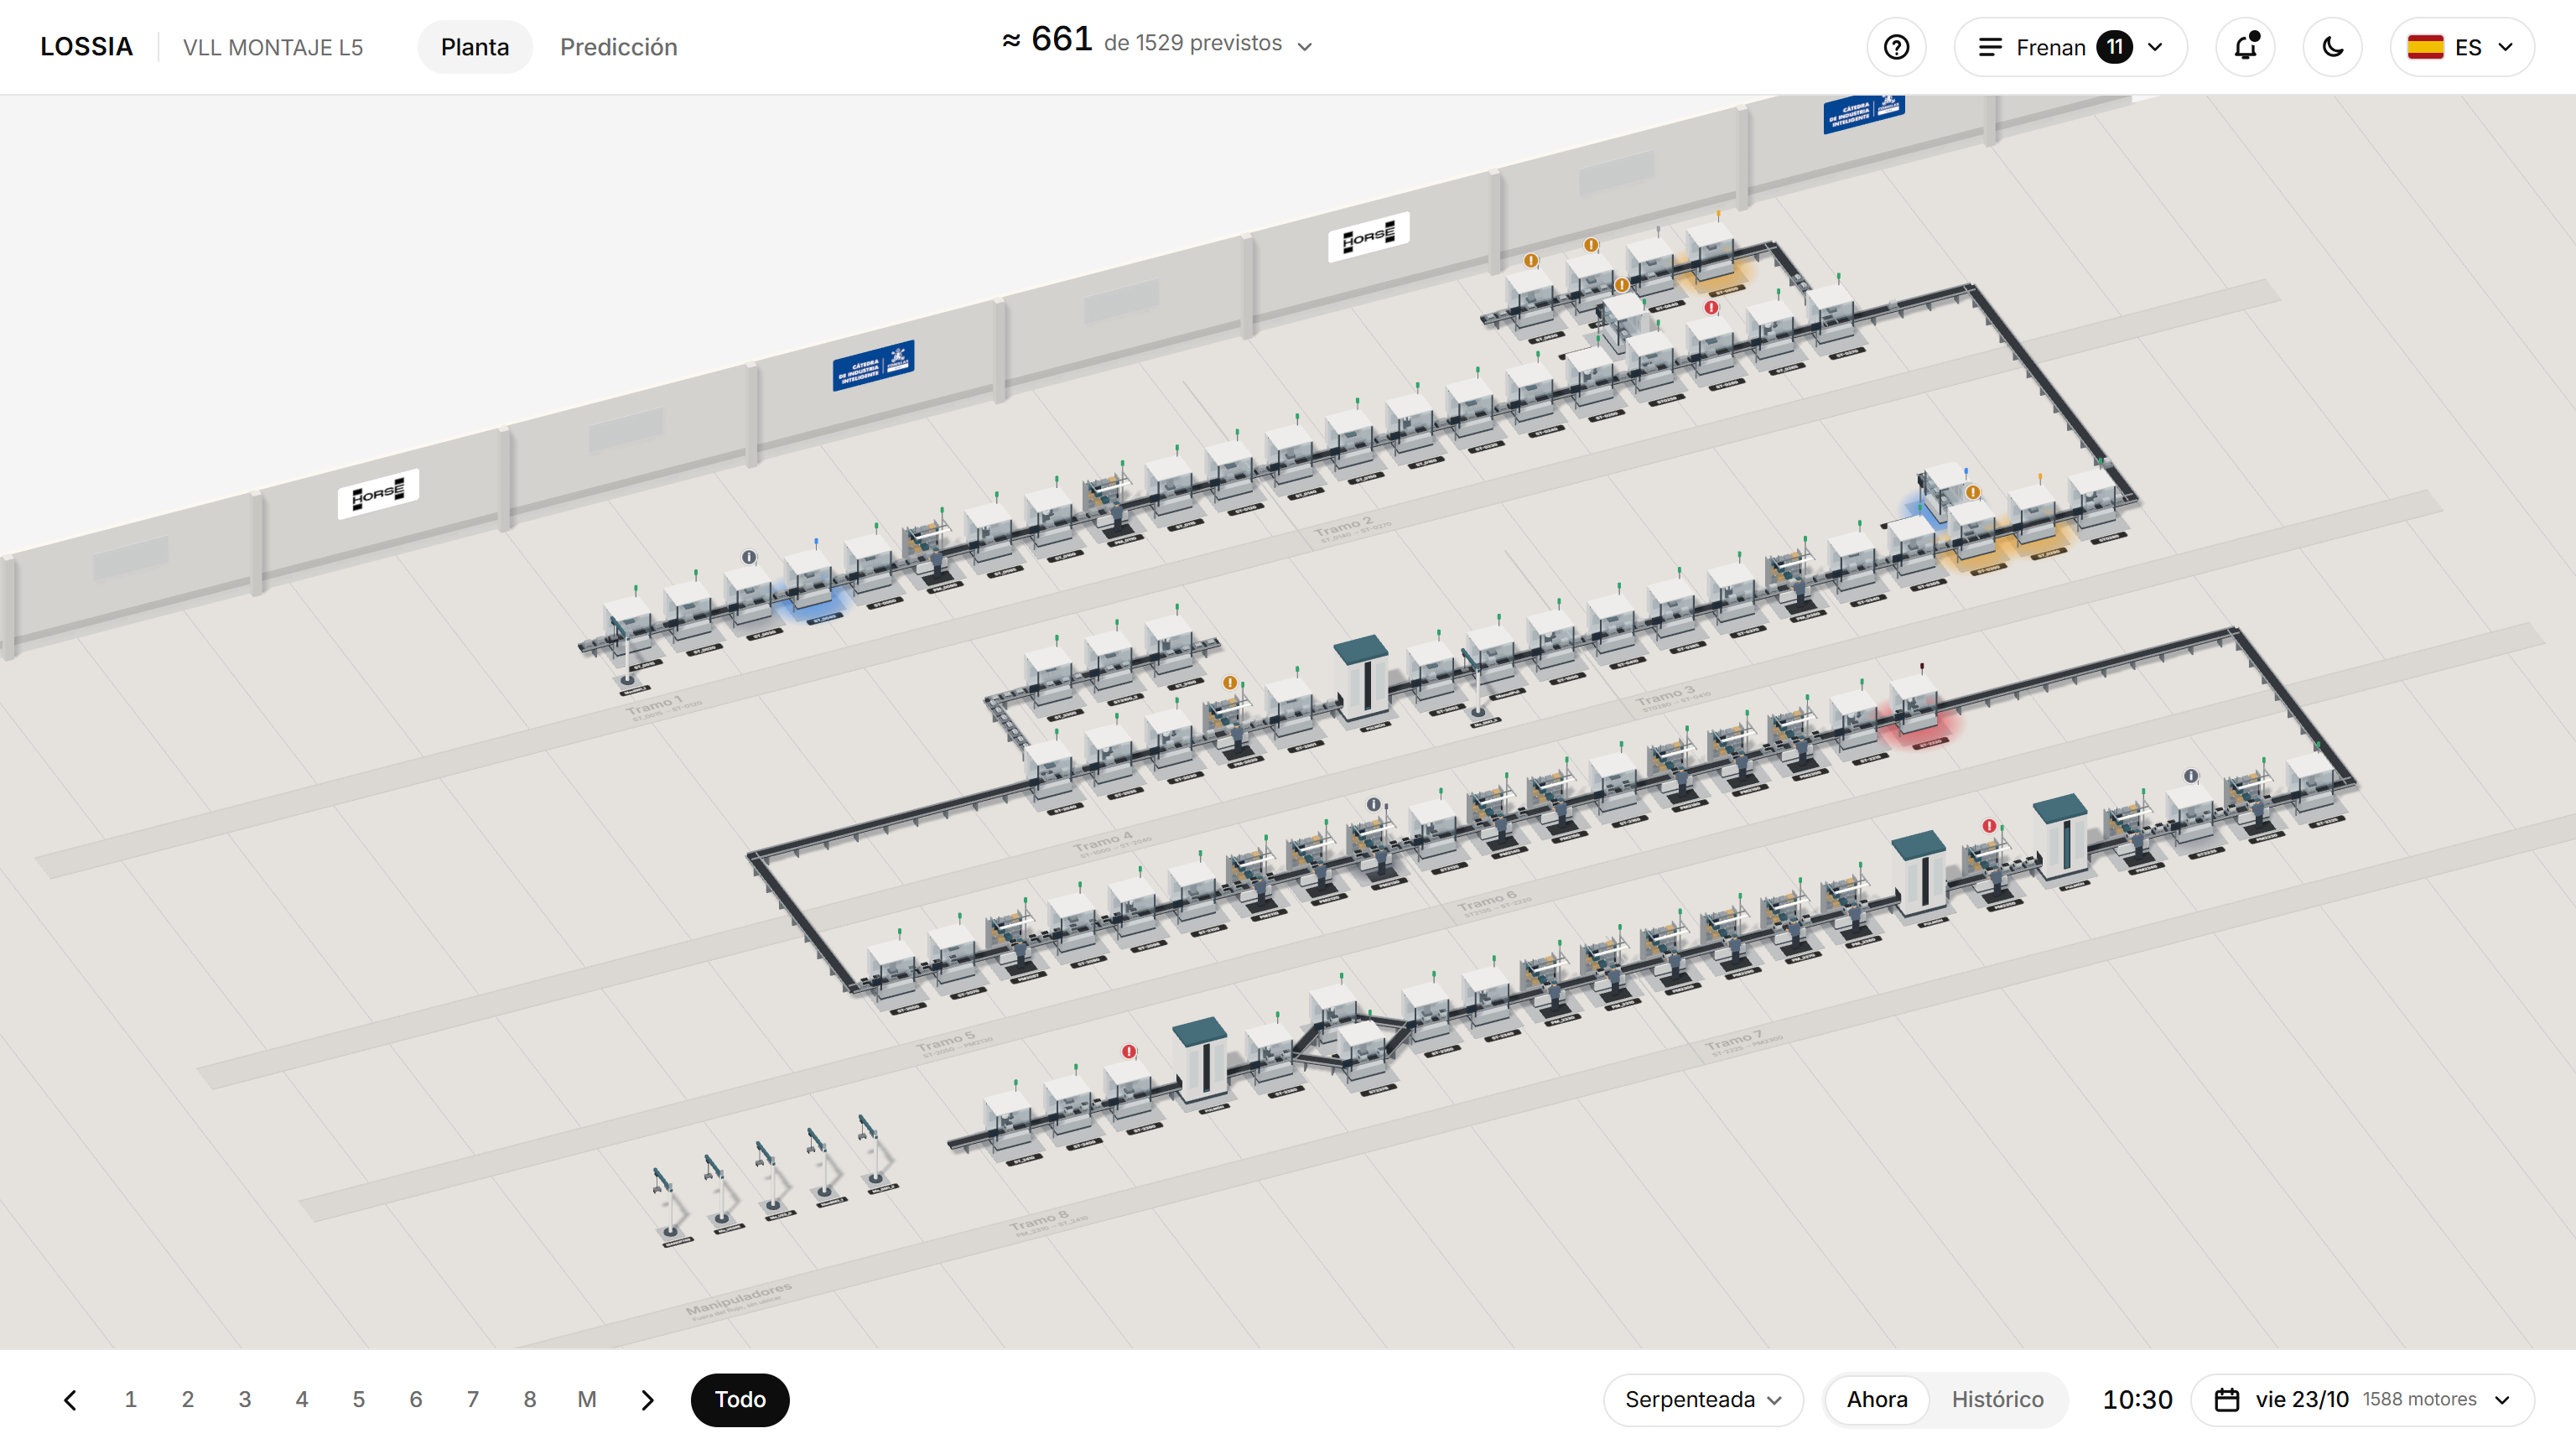
\includegraphics[width=\SW cm]{../../figures/slides/10_dashboard.png}};
  \pgfmathsetmacro{\CX}{\SX+\SW/2}
  \fill[bezel] (\CX-0.4,\SY-0.2) -- (\CX+0.4,\SY-0.2) -- (\CX+0.28,\SY-0.85) -- (\CX-0.28,\SY-0.85) -- cycle;
  \fill[bezel, rounded corners=2pt] (\CX-1.5,\SY-0.98) rectangle (\CX+1.5,\SY-0.82);
  \node[font=\Large\bfseries\color{ink}] at (\CX,\SY-1.6) {Dashboard};
  \node[font=\footnotesize\color{muted}] at (\CX,\SY-2.15) {gemelo 3D de la línea, en el navegador};
  \draw[flow] (\BR,\MY) -- (\SX-0.35,\MY);
\end{tikzpicture}
\end{document}
